% XeLaTeX编译,编译参考文献引用等需两次编译。
\documentclass[openright,oneside]{ctexbook}	% 加[draft]选项可不显示图片本体,加快编译,全文完成后再删除
\makeatletter
\renewcommand\section{\@startsection{section}{2}{\z@}%
	{1.5ex \@plus1ex \@minus.2ex}%
	{.1ex \@plus.1ex}%
	{\normalfont\normalsize\bfseries}}								%% 以上4行,定义让section后自动断行
\makeatother

	\renewcommand{\chaptermark}[1]{\markboth{第 \thechapter\ 章\quad #1}{}}
	\CTEXsetup[name={第~,~章}, nameformat={\bfseries \fangsong \zihao{4}}, titleformat={\bfseries \fangsong \zihao{4}}, number={\arabic{chapter}}]{chapter}%一级标题四号仿宋
	\CTEXsetup[beforeskip={0pt}, afterskip={20pt}]{chapter}	%章的前后行距
	
	\CTEXsetup[format={\heiti \zihao{-4}}]{section}	%二级标题四号黑体
%	\CTEXsetup[beforeskip={2ex plus .5ex minus .2sex}, afterskip={0ex plus .2ex}]{section}
	
%	\CTEXsetup[format={\fangsong \zihao{-4}}]{subsection}%三级标题小四号黑体
	%\captionwidth{0.8\textwidth}
	%\changecaptionwidth
	\CTEXoptions[contentsname={\normalfont \heiti \zihao{4}目\quad 录}, figurename={图}, tablename={表}, bibname={\zihao{-4} \normalfont \heiti 参考文献}]
	
\usepackage[titles]{tocloft}
	\renewcommand{\cftdot}{$\cdot$}
	\renewcommand{\cftdotsep}{1.5}
	\setlength{\cftbeforechapskip}{10pt}
	\renewcommand{\cftchapleader}{\cftdotfill{\cftchapdotsep}}
	\renewcommand{\cftchapdotsep}{\cftdotsep}
	\makeatletter
	\renewcommand{\numberline}[1]{%
		\settowidth\@tempdimb{#1\hspace{0.5em}}%
		\ifdim\@tempdima<\@tempdimb%
		\@tempdima=\@tempdimb%
		\fi%
		\hb@xt@\@tempdima{\@cftbsnum #1\@cftasnum\hfil}\@cftasnumb}		%% 防止目录里章节号和章节名重叠
	\makeatother
	
\usepackage{amsmath}	%[fleqn]可以公式不居中
\usepackage{amsfonts}
\usepackage{amssymb}
\usepackage{graphicx}
\usepackage[paper=a4paper, top=25 mm, bottom=20mm, left=25 mm, right=30mm, head=5 mm, headsep=2.5 mm, foot=5 mm]{geometry}
\usepackage{tabularx}
\usepackage{txfonts}
\usepackage{booktabs} % 三线表
\usepackage{multirow} % 多列
\usepackage{fancyhdr}    % 页眉页脚
\usepackage[numbers,sort&compress]{natbib}
	\setlength{\bibsep}{0ex}  % vertical spacing between references
\usepackage{algorithm}
\usepackage{algorithmic}
\usepackage{float}
	%1方式,线型
	\floatstyle{ruled}
	%2环境、浮动方式、包含文件(类似toc,lof,lot)
	\newfloat{algorithm}{htbp}{loa}[chapter]
	%3 目录名称,类似-->\renewcommand*{\lstlistlistingname}{程~序}
	\floatname{algorithm}{算~法} %环境名,使用方法\begin{algorithm}caption{}.......\end{algorithm}

\usepackage{caption}  % 标题
	\renewcommand\captionfont{\zihao{-5} \heiti}
	\captionsetup{labelsep=space}
	\captionsetup{justification=centering}
%	\captionsetup[figure]{options}
%	\captionsetup{labelsep=colon}
	\setlength{\abovecaptionskip}{6pt}
	\setlength{\belowcaptionskip}{-10pt}
	
% Windows	\newCJKfontfamily\fzyt{FZYaoTi}
% Mac \newCJKfontfamily\fzyt{FZYTK--GBK1-0}
	\newCJKfontfamily\fzyt{FZYTK--GBK1-0}

%后面有了	\setmainfont{Times New Roman}

\usepackage{enumitem}
	\setenumerate[1]{itemsep=0pt,partopsep=0pt,parsep=\parskip,topsep=0pt}
	\setitemize[1]{itemsep=0pt,partopsep=0pt,parsep=\parskip,topsep=0pt}
	\setdescription{itemsep=0pt,partopsep=0pt,parsep=\parskip,topsep=0pt}

		
	\pagestyle{plain}

	
	\newcommand{\dif}{\mathop{}\!\mathrm{d}} 

\usepackage{microtype}	%	microtype 宏包可以改善了单词、字母的间距。它可能做了很多,但是大部分人察觉不到使用它之后文档的变化。但至少,加载了 microtype 之后,文档看起来更好,也更容易阅读。注意:如果有使用到字体宏包,需要将 microtype 宏包放在它们的后面,因为这个宏包对单词、字母的调整和字体是有关的。

\usepackage{siunitx}	%	siunitx 宏包大大简化了写作科技文的 TeX 命令,科技文写作中很大一部分是单位、数字。这个宏包添加了一些命令,比如 \num命令可以输出我们想要的各种方式的数字形式(比如科学记数法),而 \si 命令用来输出单位。我经常用到的命令是 \SI 和 \SIrange。比如 \SI{10}{\hertz} 输出为 “10Hz”(这能有效避免输入错误,我可能会写成 HZ 或者 hz 而不是 Hz)。\SIrange 命令多一个参数:\SIrange{10}{100}{\hertz} 输出为 “10Hz to 100Hz”。

\begin{document}
	
	\makeatletter
	\def\@cite#1#2{\textsuperscript{[{#1\if@tempswa , #2\fi}]}}				%% 以上2行 - 把引用改上标;
	\makeatother

\begin{figure}[!htbp]
	\centering
	
\includegraphics[scale=0.11]{pic/top}
\end{figure}

\vspace{22.5pt}

\begin{center}
	{\zihao{-0} {\fzyt 本科生毕业论文(设计)}}^^^^200b \\% 这儿有个bug
\end{center}

\vspace{42.8pt}

\begin{figure}[!htbp]
	\centering
	
\includegraphics[scale=0.4244]{pic/logo}
\end{figure}

\vspace{28pt}
\setmainfont{FZYTK--GBK1-0} % 可能不用加这句,Mac下,故没尝试
\begin{flushleft}
	\zihao{3} \fzyt 
	\renewcommand\arraystretch{1.3}
	\begin{tabular}[b]{p{1.92cm}p{2.45cm}p{3.8cm}p{1.4cm}p{3.8cm}}
		& 题\hspace{2em}目:& \multicolumn{3}{c}{\underline{\makebox[10cm]{哈哈哈哈哈哈哈哈哈座蓝桑架}}} \\
		&				  & \multicolumn{3}{c}{\underline{\makebox[10cm]{标题不长不短刚刚好}}} \\
		& 姓\hspace{2em}名:& \multicolumn{3}{c}{\underline{\makebox[10cm]{某\ 某\ 某}}} \\
		& 学\hspace{2em}院:& \multicolumn{3}{c}{\underline{\makebox[10cm]{某\ 学\ 院}}} \\
		& 专\hspace{2em}业:& \multicolumn{3}{c}{\underline{\makebox[10cm]{你的专业名称}}} \\
		& 班\hspace{2em}级:& \multicolumn{3}{c}{\underline{\makebox[10cm]{专\ 业 \, 110}}} \\
		& 学\hspace{2em}号:& \multicolumn{3}{c}{\underline{\makebox[10cm]{3\,3\,3\,7\,7\,7\,9\,9}}}  \\
		& 指导教师: & \underline{\makebox[3.8cm]{导师姓名}}  & 职称: & \underline{\makebox[3.95cm]{职称}} \\
	\end{tabular}
\end{flushleft}

\vspace{\baselineskip}

\begin{center}
	\zihao{3} 	\fzyt
	\today 
	
	南京农业大学教务处制
\end{center}

\setmainfont{Times New Roman}
\thispagestyle{empty}	\setcounter{page}{0}
\clearpage


\vspace{2\baselineskip}

{\renewcommand\baselinestretch{1}\selectfont
\tableofcontents \par } \pagenumbering{Roman}	\addcontentsline{toc}{chapter}{目录}	\clearpage

\begin{center}
	\zihao{3} \heiti	南京农业大学本科生毕业论文\LaTeX 模板理工学科版本	\end{center}
\begin{center}
	\zihao{-4} \fangsong	某某某某专业学生 \quad 你的名字\\	指导教师 \quad 导师名字	\end{center}

\zihao{5}
\addcontentsline{toc}{chapter}{摘要}
\noindent{\heiti 摘要:}{\songti 本文档根据2015年本人毕业论文修改制作,读起来不顺很正常,因为我胡乱删减的。Mac下的字体是FZYTK--GBK1-0,Windows下是FZYaoTi,记得有两处要修改。对于不符合格式之处欢迎指正,请联系frankwaiichou@gmail.com} 

\addcontentsline{toc}{chapter}{关键词} 
\noindent{\heiti 关键词:}{\songti 三; 到; 五; 个; 关键词} %要具体•避免罕见缩写词和一般性词汇

\vspace{135pt}

\begin{center}
	\zihao{3} NJAU Undergraduate \LaTeX Template  S\& C Version English Title \end{center}
\begin{center}
	\zihao{-4} Student majoring in YOUR MAJOR \quad 名字\\Tutor\quad 导师\end{center}

\zihao{5}
\addcontentsline{toc}{chapter}{Abstract}
{\renewcommand\baselinestretch{1}\selectfont
\noindent\textbf{Abstract: }英文渣渣就不秀了。
	\par}

\vspace{-0.2\baselineskip}
\addcontentsline{toc}{chapter}{Key words}
\noindent\textbf{Key words: } 三; 到; 五; 个; 关键词

\vspace{15pt}
\clearpage 

\zihao{-4} \songti	

\chapter{第二章} 
\pagenumbering{arabic} % 阿拉伯数字页码

一些例子,可以模仿。

\section{引用示例}
~20~世纪~70~年代~Crosby~和~Karnopp~提出控制算法\cite{ck1,ck2,ck3}。~1986~年,~Kim~利用~lyapunov~方法行的稳定性\cite{ck2,ck3}。同年,~Choi~等人的座椅\cite{ck3}。

\section{公式示例} 
行内公示$y_{12}$、$\dot y_{12}$、$\ddot y_1$、$\dot y_1$代入得到:
{\setlength\abovedisplayskip{3pt}
	\setlength\belowdisplayskip{3pt}
	\begin{equation}	I = \left\{ {\begin{array}{*{20}{c}}
	{{K_s}|{{\dot y}_1}|}&{,{{\dot y}_1}{{\dot y}_{12}} > 0}\\
	0&{,{{\dot x}_1}{{\dot e}_{12}} \le 0}
	\end{array}} \right.	\end{equation}}

{\setlength\abovedisplayskip{3pt}
	\setlength\belowdisplayskip{3pt}
	\begin{equation}	{K_s}(k + 1) = {K_s}(k) + \mu \left[ { - \frac{{\partial P}}{{\partial {K_s}(k)}}} \right]	\end{equation}}


\section{图片示例}
此描述如图~\ref{fig1}~所示。

\begin{figure}[!htbp]
	\centering	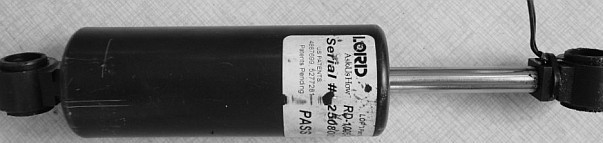
\includegraphics[width=12cm]{pic/fig1}
	\caption{长图}	\label{fig1}	\end{figure}

\begin{figure}[!htbp]
	\begin{center}
		\begin{minipage}[c]{0.44\textwidth}
			\centering		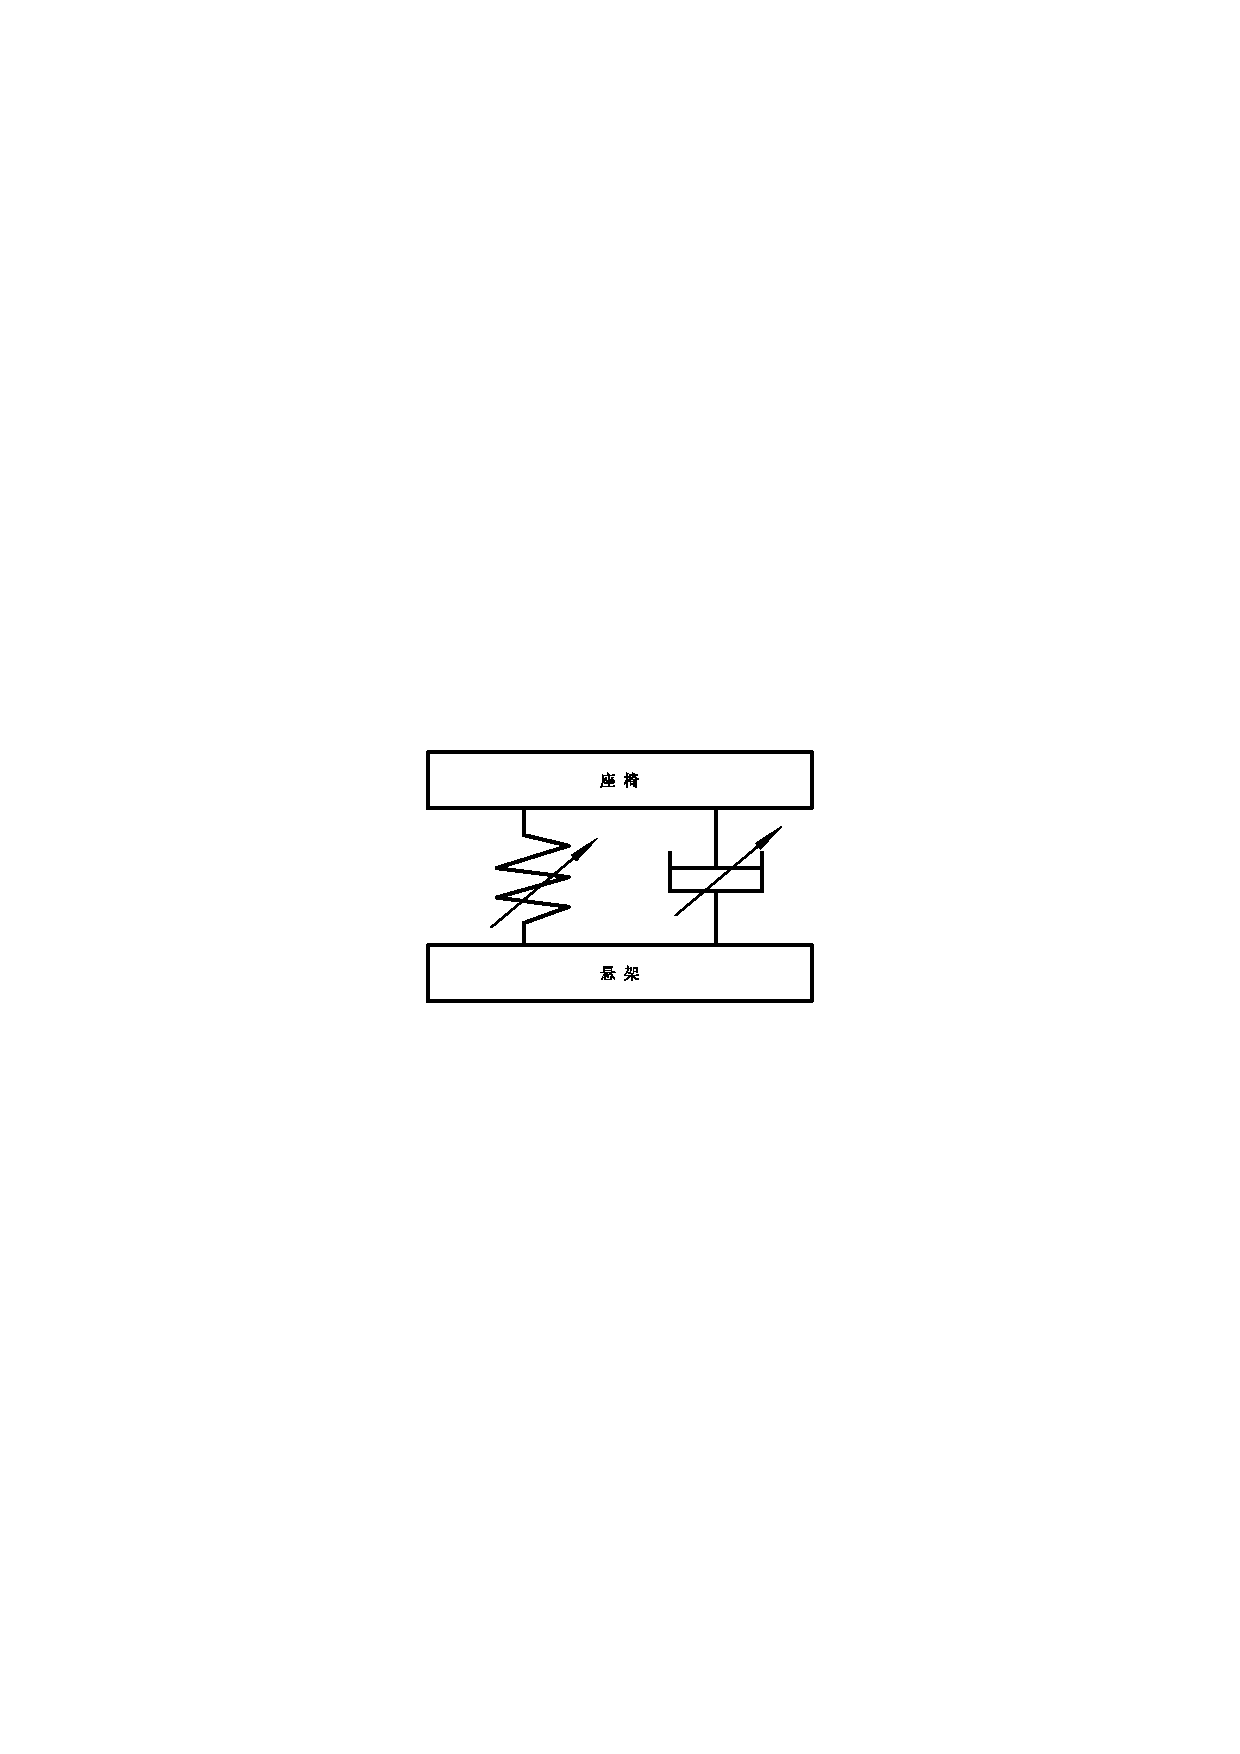
\includegraphics{pic/fig2-1}
			\caption{分图1}	\label{fig2-1}
		\end{minipage}%
		\begin{minipage}[c]{0.56\textwidth}
			\centering		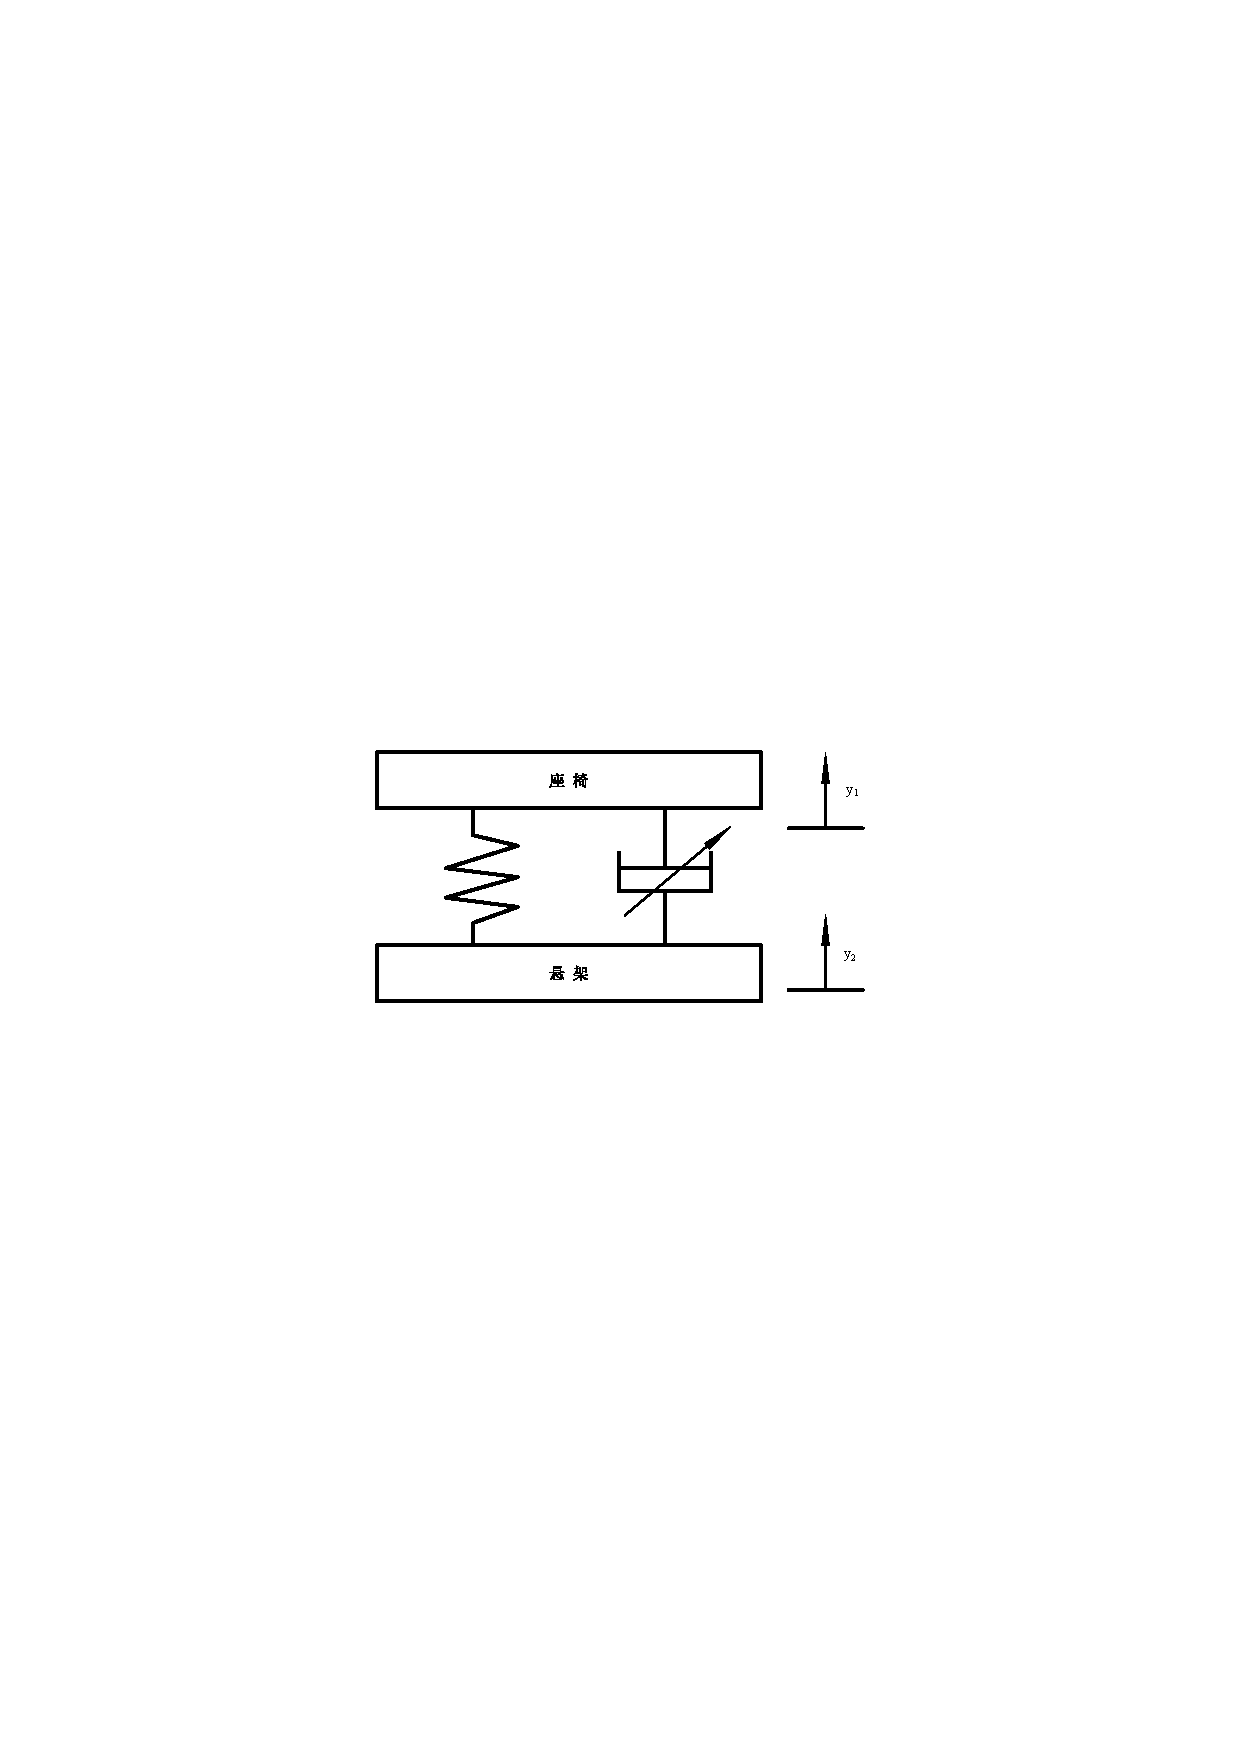
\includegraphics{pic/fig2-2}
			\caption{分图2}	\label{fig2-2}
		\end{minipage}
	\end{center}
\end{figure} 


\section{表格示例}
\begin{table}[H]
	\caption{表格示例}	\label{table1}
	\vspace{-0.5 cm} \zihao{-5}
	\begin{center}
		\begin{tabular}{cr@{.}lcr@{.}lcc}
			\toprule[1pt]
			 名  & \multicolumn{2}{c}{值} &  名  & \multicolumn{2}{c}{值} &    名     & 值 \\ \midrule[0.6pt]
			$a_0$ &  1 & 0              & $b_0$ &   2 & 73            &   $h_2$    & 0 \\
			$a_1$ &  30 & 4              & $b_1$ &   0 & 0               &   $h_3$    & 1 \\
			$a_2$ & 50 & 1              & $b_2$ &   0 & 2I+0.1          &   $h_4$    & 0 \\
			$a_3$ & -8 & 9              & $h_0$ & 111 & 1               &   $V_0$    & 0 \\
			$a_4$ & 13 & 8              & $h$ &   0 & 0               & $F_{bs}$ & 0 \\ \bottomrule[1pt]
		\end{tabular}
	\end{center}
	\vspace{-0.3 cm} \hspace{4.6 cm} {\zihao{-5} 注:此处是注释。}
\end{table}\zihao{-4} \vspace{-7pt}


\clearpage
 

%\input{Chap2} 

%\input{Chap3} 

%\input{Chap4} 

\addcontentsline{toc}{chapter}{参考文献}
\zihao{5}
%\bibliographystyle{gbt7714-2005}
%\bibliography{my.bib}

%完成后再改成thebib...
\begin{thebibliography}{99}
\bibitem{ck1} Crosby M J, Karnopp D C. System for controlling the transmission of energy between spaced members: U.S. Patent 3,807,678[P]. 1974-4-30.
\bibitem{ck2} Crosby M J, Karnopp D C. System for controlling the transmission of energy between spaced members: U.S. Patent 3,807,678[P]. 1974-4-30.
\bibitem{ck3} Crosby M J, Karnopp D C. System for controlling the transmission of energy between spaced members: U.S. Patent 3,807,678[P]. 1974-4-30.
\end{thebibliography}

\end{document}
